\chapter{DEAP}
\label{chap:DEAP}
\textbf{D}ark matter \textbf{E}xperiment with liquid \textbf{A}rgon \textbf{P}ulse shape discrimination (\gls{deap}) is an argon nuclei based noble liquid direct dark matter detection project designed to detect WIMP induced scintillation. In this chapter the detection process that \gls{deap} uses is described as well as the detector's construction.

\section{Scintillation}

\subsection{Noble Gas Scintillators}
Scintillation is a light emitting interaction that occurs in certain materials known as scintillators. Incident radiation or particles that deposit energy in the scintillator cause the release of scintillation light. In liquid noble gases, when a nuclei is excited or ionized, they can form strong bonds with a ground state atom to form either an ionized or excited dimer state known as excimers \cite{mullikenNobleScintillation}. These excimers are metastable and will radiatively decay. A diagram for a particle interaction producing scintillation light in argon is shown in Fig. \ref{Fig:scintillation}.
\begin{figure}[ht]
\centering
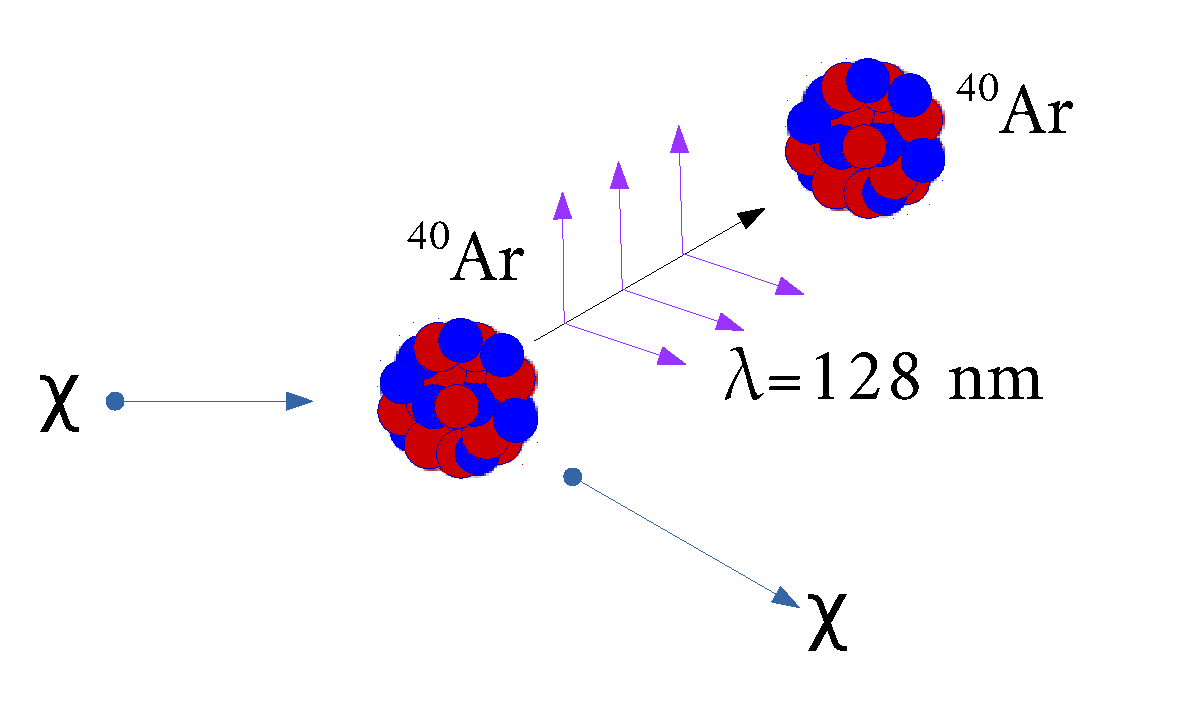
\includegraphics[height = 0.17\paperheight]{scintillation}
\caption{DEAP senses particle interactions through the release of ultraviolet light caused by the nuclear or electronic recoil of the argon nuclei.}
\label{Fig:scintillation}
\end{figure}

Noble liquids are attractive medium choices in particle detectors due to their relatively low price, high light yield, scalability, and self-shielding ability. Of the noble liquids, neon, argon, krypton, and xenon have potential for use and have been used in other \gls{wimp} detectors such as LUX \cite{LUX2015Results} and XENON \cite{XENON100}. Argon was chosen for a combination of reasons especially its high light yield, potential for single stage detection (see Section \ref{sec:PSD}), and low cost \cite{2004BouleyPSD} \cite{deap3DarkMatterSearch} \cite{argonScintillation}.

\begin{table}
\centering
\caption{Properties of the noble gases \cite{chemicalHandbook}. Note prices are approximate and vary based on source and purity levels.}
\begin{tabular}{l	c	c	c	c	c	c}
\hline
\hline
Property&			He&		Ne&		Ar&		Kr&		Xe&		Rn\\
\hline
Atomic Number&				2&		10&		18&		36&		54&	86\\
Atmospheric ppm&			5&		15.4&	9400&	1&		$\frac{1}{20}$&	10$^{-15}$\\
Cost per kg (CAD\$)& 				52.00&	330.00&	5.00&	330.00&	1200.00&	-\\
Melting Point T$_{m}$ (K)&	-&		24.6&	83.8&	115.8&	161.4&	202.0\\ 
Boiling Point T$_{b}$ (K)&	4.22&	27.07&	87.29&	119.92&	165.10&	211.3\\
\hline
\hline
\end{tabular}
\label{Table:nobleCharacteristics}
\end{table}





Argon excimer formation occurs when an argon atom in atomic state $^3$P$_{1}$ or $^3$P$_{2}$ bonds with one in the $^1\text{S}_{0}$, or ground, state. There are therefore, two possible spin configurations for a dimer pair: a singlet state, \gls{singlet}$(^3\text{P}_{1} \ + \ ^1\text{S}_{0})$, or a triplet state, \gls{triplet}$(^3\text{P}_{2} \  + \ {^{1}\text{S}_{0}})$ \cite{mullikenNobleScintillation}. Both configurations are metastable and will decay releasing 128 nm vacuum ultraviolet light (\gls{vuv}) as depicted in Fig. \ref{Fig:decayStates}. There is no long lasting chemical change to the argon after an interaction.


\begin{figure}[ht]
\centering
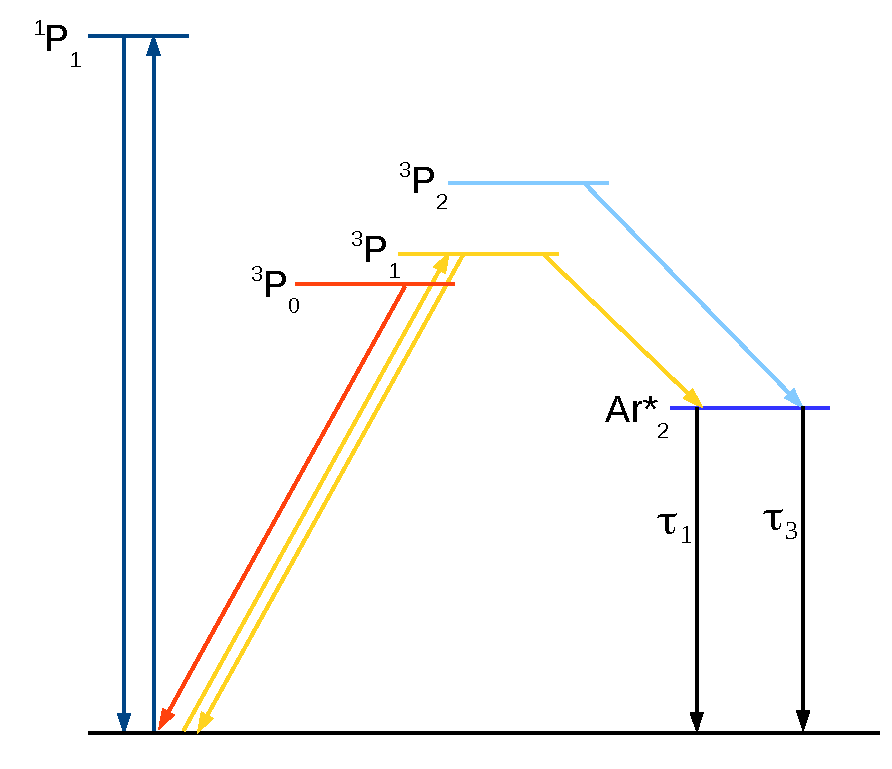
\includegraphics[height = 0.25\paperheight]{energyLevels}
\caption{Diagram of the energy level of the first few argon atomic states with the potential increasing with height (image based on \cite{tinaPollmann} and \cite{UVEmissionInArgon}). The emitted photon from the excimer decay has a lower energy than any atomic absorption line, ensuring that it will not be reabsorbed in the medium.}
\label{Fig:decayStates}
\end{figure}

Eximers can be formed through one of two mechanisms: direct excitation or ionization. Excitation occurs when one of the $^3$P$_{1}$ or $^3$P$_{2}$ atomic states forms a strong bond to a ground state atom which then radiatively decays \cite{1983HitachiXenonAndArgonLuminesince}: 
\begin{equation}
\begin{split}
\text{Ar}^{*} + \text{Ar} &\rightarrow \text{Ar}_{2}^{*}\\
\text{Ar}_{2}^{*} &\rightarrow 2\text{Ar} + \text{h}\nu .
\end{split}
\label{Eq:exiteDecay}
\end{equation}

If an ion is produced, it must first recombine with a free electron and (non-radiatively) decay to one of the allowed excited states before forming an excimer and producing a scintillation photon:

\begin{equation}
\begin{split}
\text{Ar}^{+}+\text{Ar} &\rightarrow \text{Ar}_{2}^{+}\\
\text{Ar}_{2}^{+} + e^{-} &\rightarrow \text{Ar}^{**} + \text{Ar}\\
\text{Ar}^{**} &\rightarrow \text{Ar}^{*} + \text{heat}\\
\text{Ar}^{*} + \text{Ar} &\rightarrow \text{Ar}_{2}^{*}\\
\text{Ar}_{2}^{*} &\rightarrow 2\text{Ar} + \text{h}\nu .
\end{split}
\label{Eq:ionizeDecay}
\end{equation}



Both ionization and direct excitation of argon can cause the formation of triplet (\gls{triplet}) and singlet (\gls{singlet}) state excimers. The \gls{singlet} state follows an allowed transition of \gls{singlet} $\text{Ar}_{2}^{*} \rightarrow 2\text{Ar} + \text{h}\nu$ and does so in a characteristic time, $\tau_1$. The \gls{triplet} state decay is dipole-forbidden and therefore has a longer characteristic decay time $\tau_3$, the values of which are given in Table. \ref{Table:scintTime}. This difference in the state decay time gives the characteristic slow and fast light observed after a particle interaction in argon \cite{1983HitachiXenonAndArgonLuminesince}. Both argon and neon share this large time separation, which makes them excellent candidates for single stage scintillation detectors based on pulse shape discrimination (Section \ref{sec:PSD}). The characteristic lifetimes of the two states for different noble liquids are summarized in Table. \ref{Table:scintTime}.

\begin{table}
\centering
\caption{Characteristic decay lifetimes of the singlet and triplet states in the common noble liquids \cite{argonScintillation}.}
\begin{tabular}{l	c	c}
\hline
\hline
&	Singlet $\tau_1$ (ns)&	Triplet $\tau_3$ (ns)\\
\hline
Neon&	18.2 $\pm$ 0.2&	14900 $\pm$ 300\\
Argon&	7.0 $\pm$ 1.0&	1600 $\pm$ 100\\
Xenon&	4.3 $\pm$ 0.6&	22.0 $\pm$ 2.0\\
\hline
\hline
\end{tabular}
\label{Table:scintTime}
\end{table}


%\clearpage
\subsection{Pulse-shape Discrimination}
\label{sec:PSD}

Any scintillation producing interaction will produce both triplet (\gls{triplet}) and singlet (\gls{singlet}) state excimers, the proportions of which are set by the linear energy transfer, dE/dx, (\gls{let}) of the incident particle or radiation. A higher \gls{let} deposits more energy over a given distance producing more \gls{singlet} states \cite{LETArgonDependance}. Electronic events are not as easily absorbed as nucleons, causing a much lower \gls{let} for electronic events and therefore a great disparity in the \gls{singlet} to \gls{triplet} states produced. Using these properties it is possible to separate events into electronic events ($\gamma$ or $\beta$) from nucleon events (neutron, $\alpha$, or \gls{wimp}) by looking at the timing distribution in the events' scintillation light; the proportion of states is shown in Table. \ref{Table:singletTripletProportions}. By looking at the timing of the scintillation from an event, important information about the event type can be deduced. This process known as pulse-shape discrimination (\gls{psd}) has been shown by the DEAP/CLEAN collaboration to be an accurate metric for distinguishing between nuclear recoils and electromagnetic events \cite{2004BouleyPSD}.

\begin{table}
\centering
\caption{Intensity proportion of singlet to triplet states produced in liquid Ar $\&$Xe \cite{1983HitachiXenonAndArgonLuminesince}.}
\begin{tabular}{l	c	c	c}
\hline
\hline
&	Electrons (I$_s$/I$_t$)&	$\alpha$s (I$_s$/I$_t$)& 	Fission Products (I$_s$/I$_t$)\\
\hline
Argon&	0.3&	1.3&	3.0\\
Xenon&	0.05&	0.45$\pm$0.07&	1.6$\pm$0.2\\
\hline
\hline
\end{tabular}
\label{Table:singletTripletProportions}
\end{table}

As a proxy for measuring the \gls{let} of an event, the fraction of prompt light is used as it is sensitive to changes in the \gls{let} of an event while being simple to measure. This quantity is known as \gls{fprompt}. The larger proportion of longer lived \gls{triplet} states in $\gamma$ or $\beta$ events means a lower \gls{fprompt} than that of a nuclear recoil event. The significant difference in the decay time between states in argon (see Table. \ref{Table:scintTime}) allows for the determination of the incident particle type from the events prompt charge and \gls{fprompt} alone \cite{2004BouleyPSD}. 

\gls{fprompt} is calculated by integrating the resulting charge about the primary peak in a short time window ($\tau_{short}$) and dividing that by the charge in a much longer time interval ($\tau_{long}$):

\begin{equation}
\frac{\int_{0}^{\tau_{short}} f(t) dt}{\int_{0}^{\tau_{long}} f(t) dt}
\label{Eq:fpromptDefinition}
\end{equation}
The current \gls{deap3} short and long window durations are 140 ns and 6000 ns respectively.

A plot of calibration events depicting the \gls{fprompt} event separation from the \gls{deap1} prototype is shown in Fig. \ref{Fig:deap1Fprompt}. This method of \gls{psd} using \gls{fprompt} is the same as to be used in \gls{deap3}. The accurate separation between electronic and nuclear recoil events is crucial in argon based detectors due to the natural occurrence of $^{39}$Ar in atmospheric argon which causes a $\beta$-decay background at a 1 Hz/kg rate. \gls{deap3} has two levels of \gls{psd}, a course background reduction level and a more precise version done in data analysis once the event has been saved to disk. The introduction of the \gls{psd} based trigger to mitigate these events is extensively covered in Chapter \ref{chap:triggerDesign}.

\begin{figure}[ht]
\centering
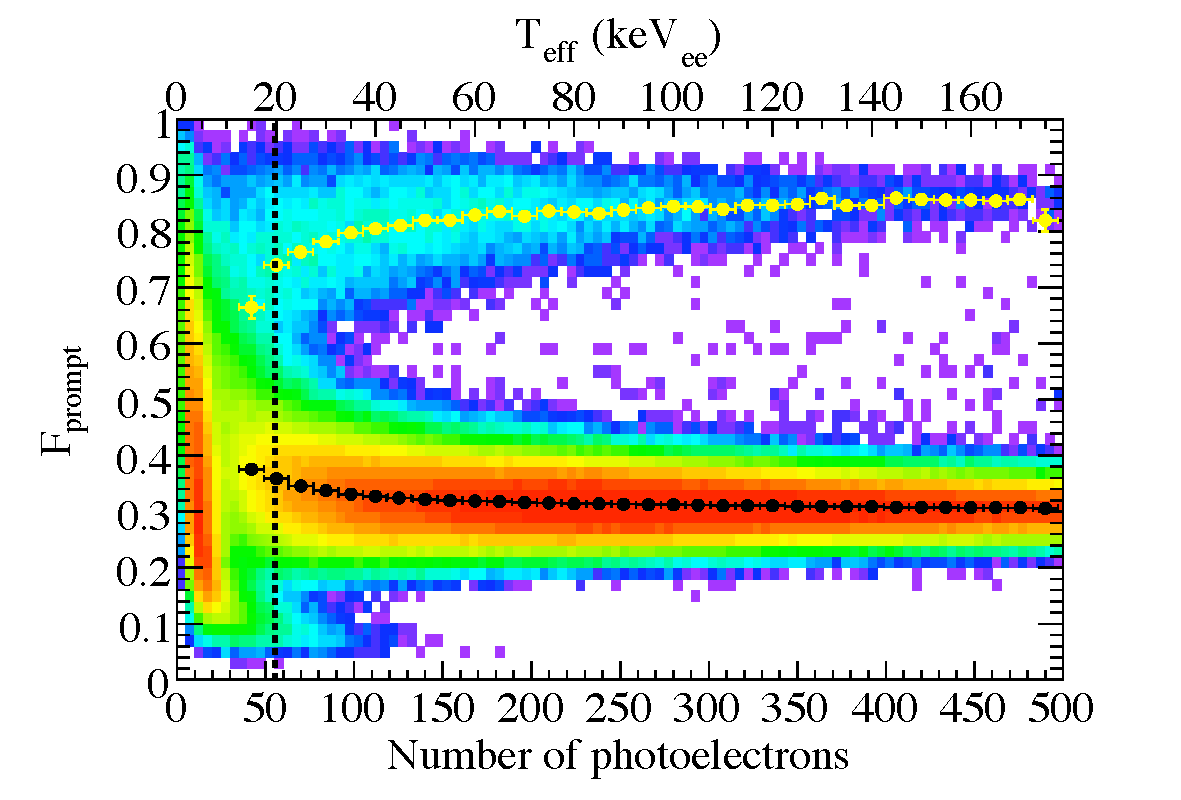
\includegraphics[height = 0.26\paperheight]{Deap1Data}
\caption{\gls{deap1} Fprompt and energy distribution of neutron and $\gamma$ argon scintillation events from an Am-Be calibration source. Nuclear recoils from incident neutron are in the upper band (yellow), the lower band (black) is that of $\gamma$-ray interactions. It is this separation between event types that allows for background suppression of $\beta$ $\&$ $\gamma$ events in \gls{deap3}.}
\label{Fig:deap1Fprompt}
\end{figure}


%\clearpage
\section{DEAP Detectors}
The \gls{deap} experiment uses a single phase \gls{psd} detection scheme whereby scintillation is the only signal detected as previously discussed. The predecessor to \gls{deap3} was the \gls{deap1} prototype detector which established the construction techniques and background mitigation used in \gls{deap3} \cite{tinaPollmann}. The \gls{deap1} detector, shown schematically in Fig. \ref{Fig:deap1Rendering}, has been operating since 2006.

\begin{figure}[ht]
\centering
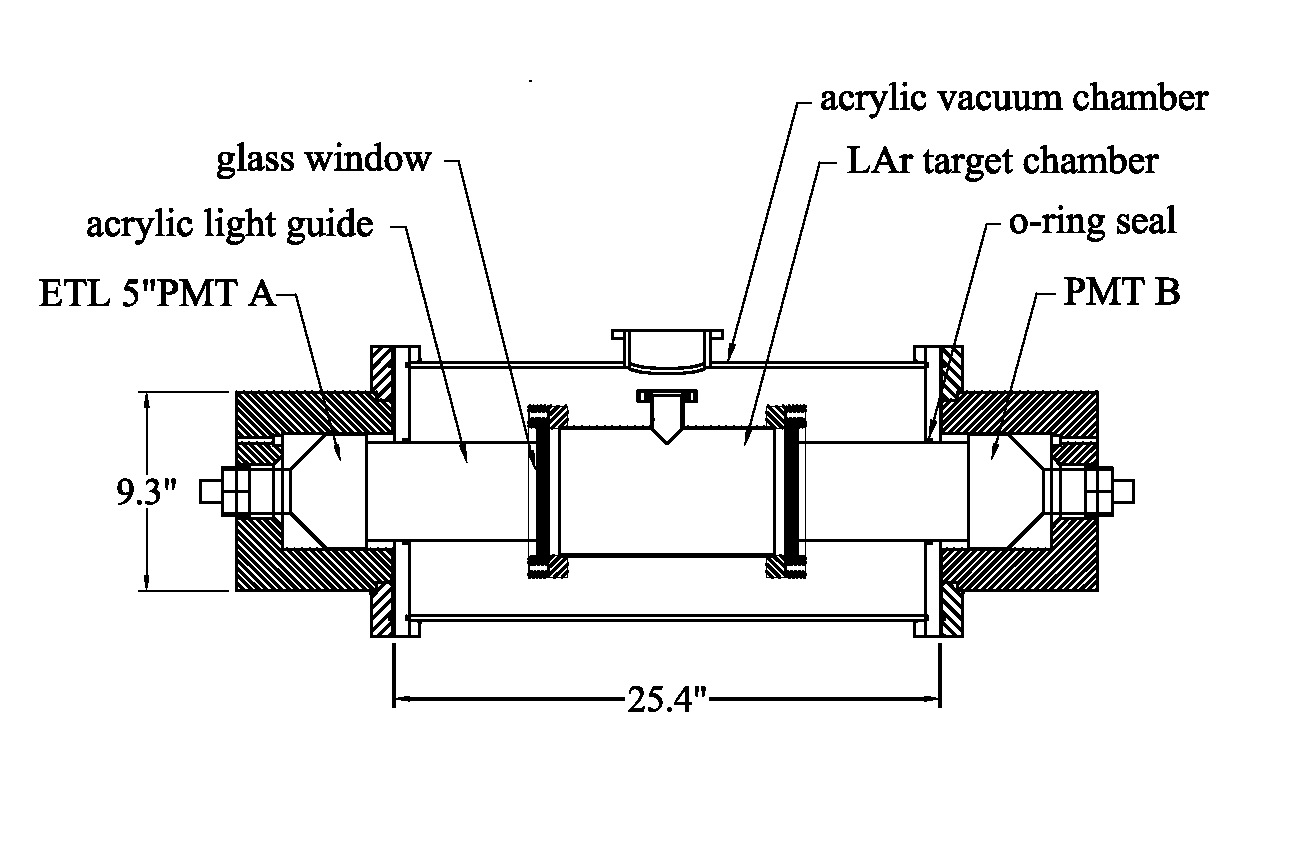
\includegraphics[height = 0.3\paperheight]{deap1_tag}
\caption{Schematic design of the \gls{deap1} detector configuration. Liquid argon is held within the central stainless steel chamber.  The chamber is lined with an inner acrylic cylinder and a diffuse reflector. \gls{tpb} is coated on the inner detector surface to wavelength-shift the scintillation light from 128 nm $\rightarrow$ 425 nm. The shifted light is transmitted to the \gls{pmt}s through \gls{pmma} (polymethyl methacrylate) acrylic light guides, thermally insulating the \gls{pmt}s and shielding the argon from any neutron sources in the \gls{pmt}s. The latest version of \gls{deap1} is outfitted with the same \gls{pmt}s as used with \gls{deap3}. Image from: \cite{2009DEAP1}.}
\label{Fig:deap1Rendering}
\end{figure}

\gls{deap3}, the second \gls{deap} collaboration detector now nearing completion, succeeds the \gls{deap1} proof of concept design. The primary sections of the detector from early construction are shown in Fig. \ref{Fig:detectorBalls}; Fig. \ref{Fig:deap3Rendering} shows a rendering of the detector with its main components labelled.


\begin{figure}[ht]
\centering
\begin{minipage}{0.31\textwidth}
\includegraphics[width = \textwidth]{avRound}
%\caption{\gls{deap1} }
%\label{Fig:avBall}

\end{minipage}
\begin{minipage}{0.31\textwidth}
\includegraphics[width = \textwidth]{pmtBallRound}
%\caption{\gls{deap1} }
%\label{Fig:pmtBall}

\end{minipage}
\begin{minipage}{0.31\textwidth}
\includegraphics[width = \textwidth]{ballImageRound}
%\caption{\gls{deap1} }
%\label{Fig:steelBall}

\end{minipage}
\caption{\textbf{Left:} The acrylic vessel with light guides attached. \textbf{Center:} Detector with \gls{pmt}s $\&$ foam/filler blocks installed. \textbf{Right:} Detector with steel shell and outward facing veto \gls{pmt}s installed.}
\label{Fig:detectorBalls}
\end{figure}


\begin{figure}[ht]
\centering
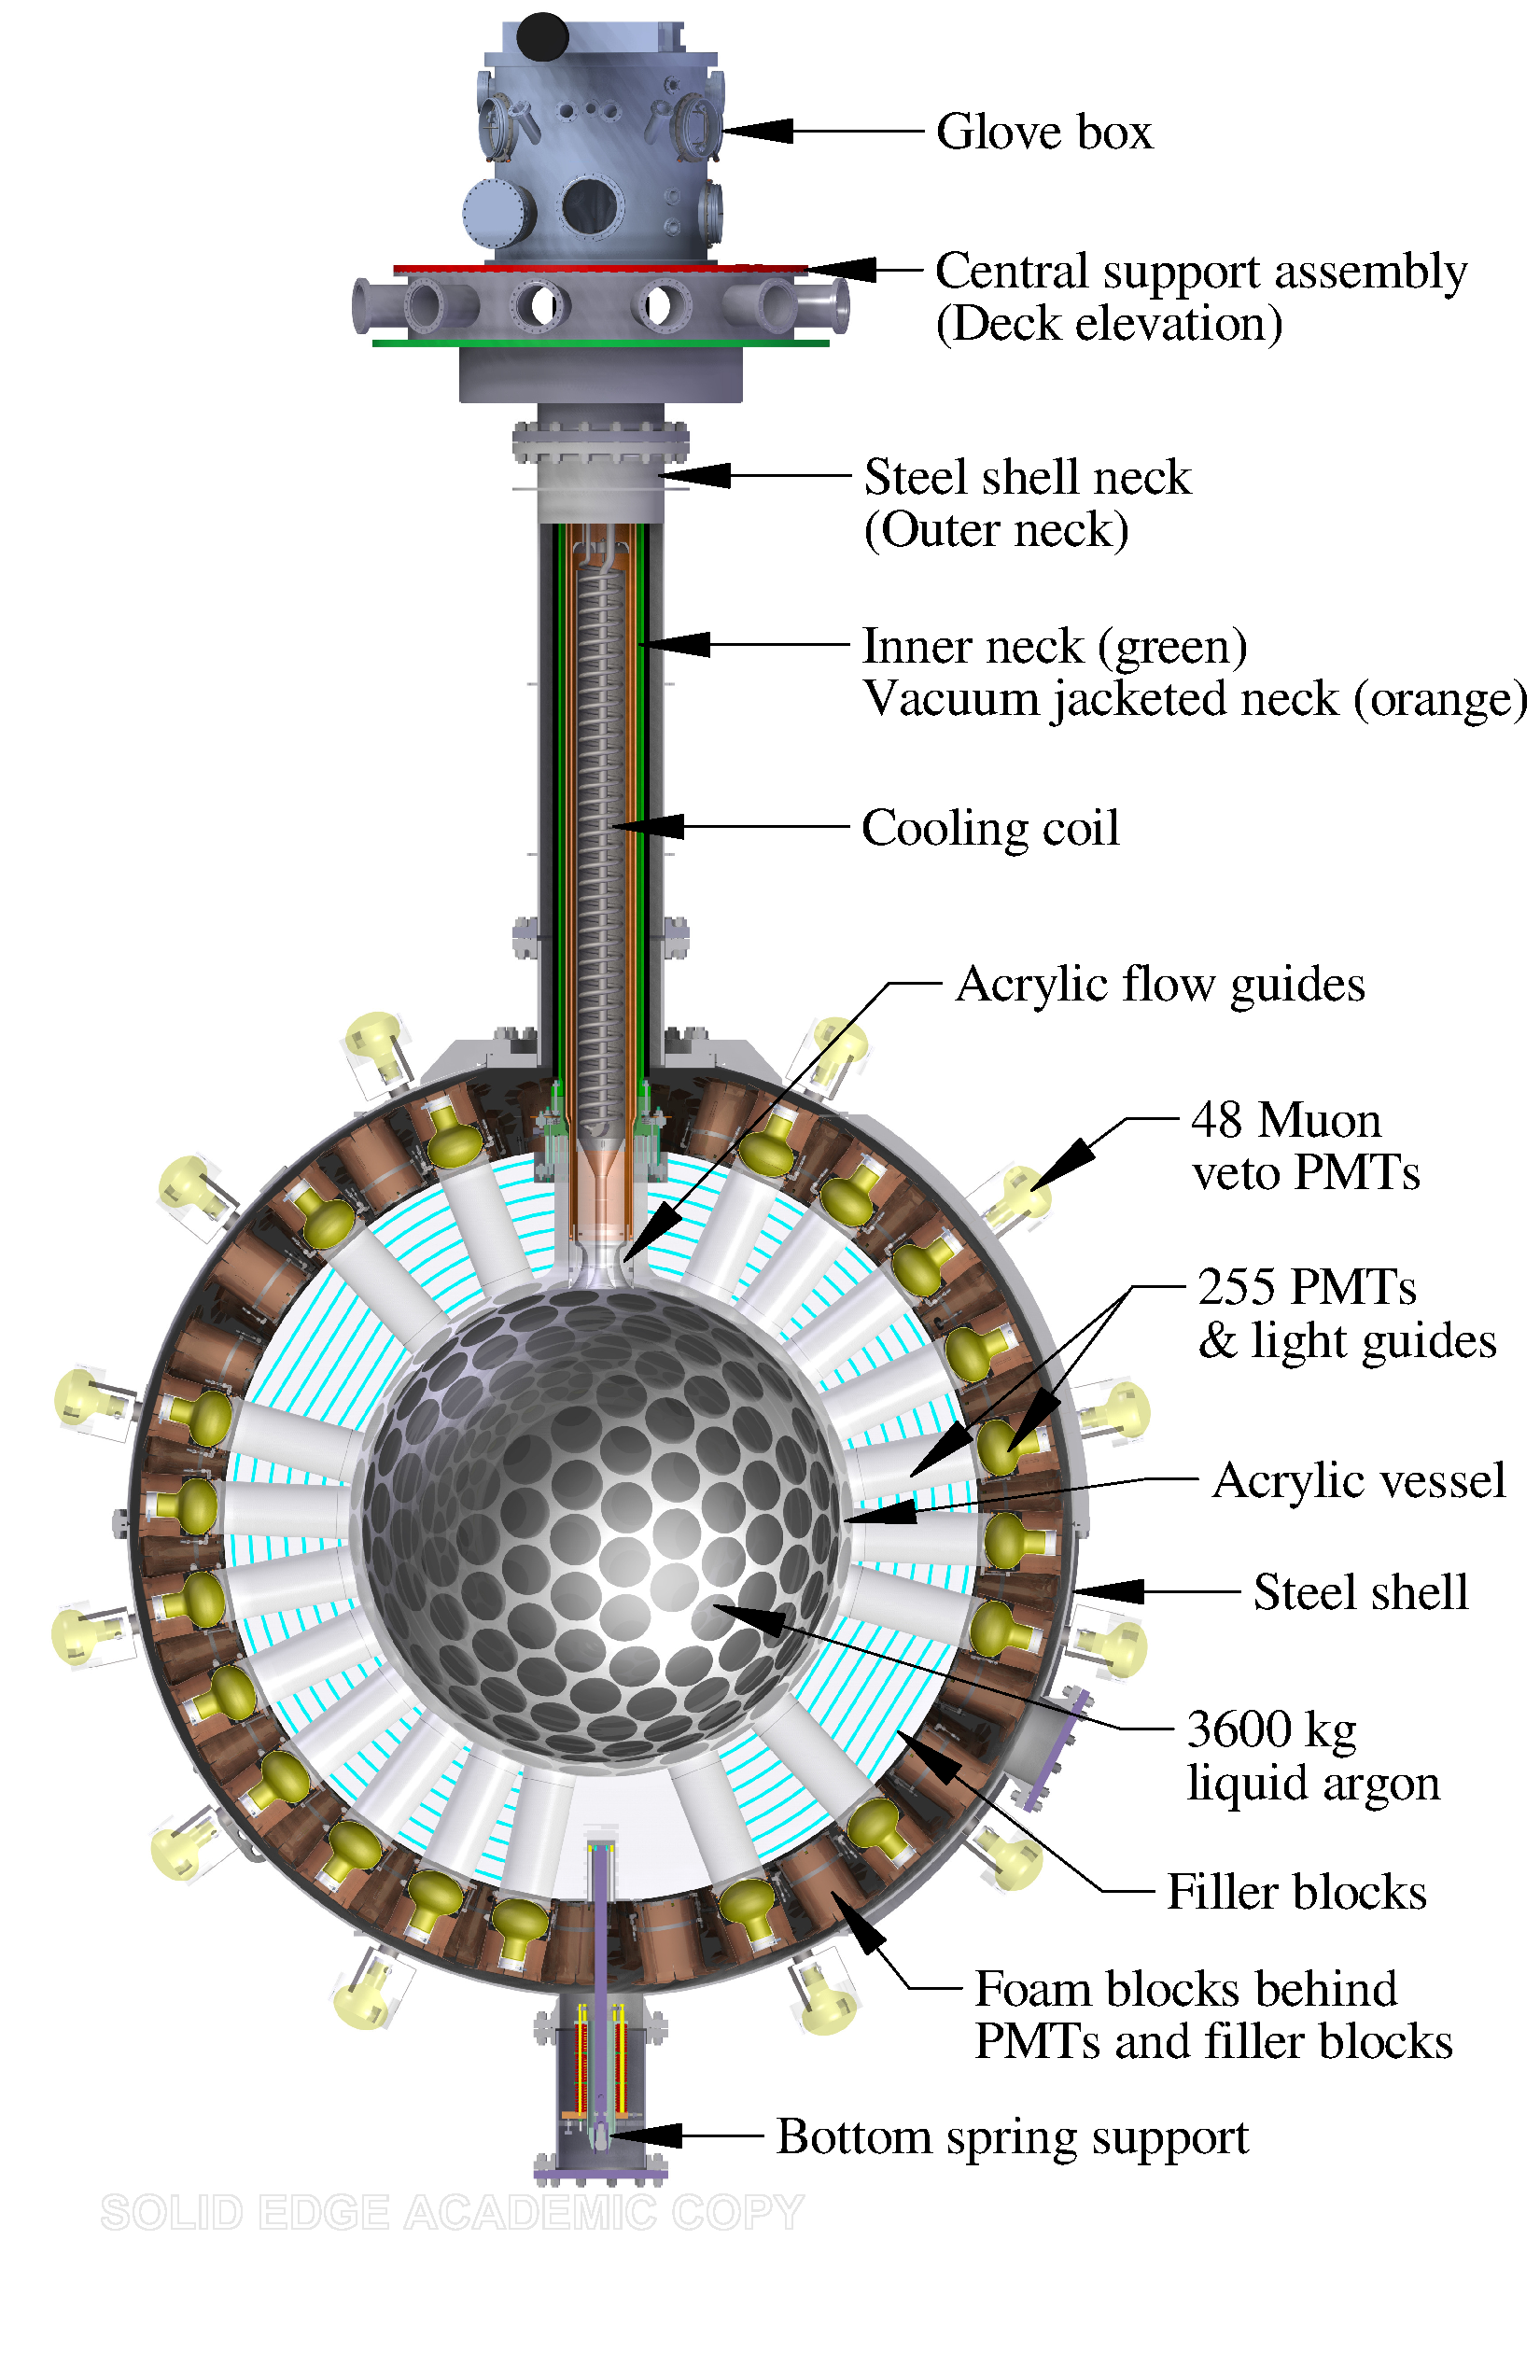
\includegraphics[height = 0.7\paperheight]{OverviewFigure}
\caption{Engineering design rendering of the \gls{deap3} detector. Each of the primary components are labeled.}
\label{Fig:deap3Rendering}
\end{figure}


The detector is located 2 km underground in Sudbury, Ontario at \gls{snolab} which provides 6010 meters of water equivalent (\gls{mwe}) shielding, reducing the cosmogenic muon flux. The 2-inch thick ultra-clean inner acrylic vessel (\gls{av}) is 170 cm in diameter and holds 3.6 tonnes of liquid argon. Events that occur near the surface are removed leaving a final fiducial volume of 1000 kgs in the central detection zone. The \gls{av} is coated with the wavelength shifter \gls{tpb}, which is required for the \gls{pmt} detection. Light guides are attached to the \gls{av} which serve to insulate the \gls{pmt}s from the target mass allowing a higher operating temperature. The light guides also serve as neutron absorbers along with the high density polyethylene filler material. A total of 255 inward-facing, eight-inch Hamamatsu R5912 high quantum efficiency photo multiplier tubes (\gls{pmt}s) are used for detection and are each attached to a PMMA (polymethylmethacrylate) light guide. A stainless steel shell surrounds the \gls{av} acting as both support and as to seal the container. The detector is housed in a 8-meter diameter water tank to provided additional shielding. There are 48 Hamamatsu 1408 \gls{pmt}s attached to the detectors exterior that are used to veto any Cherenkov light caused by incident muons (primarily from decays within the mine) \cite{tinaPollmann}. The veto system and the water tank act as both a passive shield and as an active rejection system for any surviving cosmogenic or subterranian muons. Construction of \gls{deap3} is complete. Cool-down and argon-filling is currently underway.

The hyper-sensitivity of \gls{deap3} depends upon the low background possible, which is predicted to be about 0.6 events from all sources in the \gls{wimp} region of interest over 3 tonne-years. The detector's location at \gls{snolab}, with a 6010 m.w.e overburden, is well shielded from cosmogenic muons and the water tank and active muon veto system aids in further muon rejection. Materials were chosen to be low in neutron or alpha sources, all materials being prepared in low-radon environments. An in-depth discussion on the preparation of low background components is covered in Ref. \cite{deap3DarkMatterSearch}. The total expected event rates for \gls{deap3} are given in Table \ref{Table:backgrounds}.


\begin{table}
\centering
\caption{Expected event rates in the \gls{deap3} detector at \gls{snolab} \cite{DEAP3atSNOLAB2012}.}
\begin{tabular}{l	l}
\hline
\hline
Event&										Rate (Hz)\\ 	
\hline	
$^{39}$Ar $\beta$-decay&					{$3.6 \times 10 ^{3}$}\\
Surface Background&							$< 10^{-3}$\\
Cosmic Muons&								$< 10^{-3}$\\
{WIMPs}&									{$< 10^{-5}$}\\
$^{222}$Rn decay&							$< 5 \times 10^{-6}$\\
Neutron Sources in Ar&						$< 10^{-6}$\\
\hline
\hline
\end{tabular}
\label{Table:backgrounds}
\end{table}


The dominant background will be that of naturally occuring $^{39}$Ar $\beta$-decay at a rate of $\sim$1 Hz/kg of atmospheric argon. The $\beta$-decay events cause electronic recoils in the argon and can be separated from any nuclear recoil events using \gls{psd}. Due to the high proportion of $\beta$ events to expected \gls{wimp} events (a difference of 10$^8$), it is important to suppress $\beta$ events at the trigger level. \gls{psd} reduction of $\beta$ events by the trigger will minimize dead time as the digitizers will not record for all of these events. Trigger level background mitigation will also decrease the bandwidth and storage requirements of the data acquisition system (\gls{daq}). The trigger algorithm is discussed in depth in the next chapter.